\scanpage{34}\mspage{VIII}
Comme $]s,s'[\subset\mathbb{R}^{2}-\Gamma$ est connexe on a $]s,s'[\subset\operatorname{int}\Gamma$ ou bien $]s,s'[\subset\operatorname{ext}\Gamma$.

Si $t^{\deleted{\unsure{*|'}}}\in ]s,s'[$ alors $t\in\alpha\subset\partial E(\Gamma)$ \inserted{et \deleted{\unsure{donc}} $t\in\mathbb{R}^{2}-\Gamma$,} Comme $\partial E(\Gamma)$ est un polygone convexe il vérifie la condition b) de la definition 1 (cf. lemme VI), on peut donc choisir $D_t\subset\mathbb{R}^{2}-\Gamma$ satisfaisant b). Mais $D_t\cap\operatorname{ext}\partial E(\Gamma)\ne\phi$ \inserted{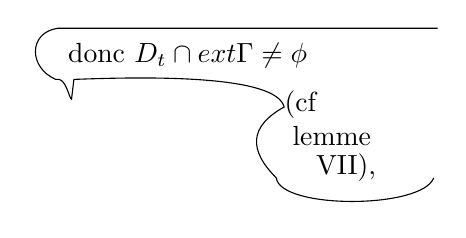
\begin{tikzpicture}[x=1cm,y=1cm,baseline=(line.base)]
\node[anchor=west,inner sep=0pt] (line) at (0,0) {donc $D_t\cap\operatorname{ext}\Gamma\ne\phi$};
\node[anchor=west,inner sep=0pt] at (2.75,-.62) {(cf};
\node[anchor=west,inner sep=0pt] at (2.85,-1.02) {lemme};
\node[anchor=west,inner sep=0pt] at (3.15,-1.42) {VII),};
\draw (4.7,.35)--(-.12,.35) .. controls (-.5,.3) and (-.5,-.15) .. (-.15,-.3)
 .. controls (-.02,-.26) and (.02,-.55) .. (.05,-.55)
 --(.08,-.3) .. controls (1.1,-.26) and (2.65,-.25) .. (2.75,-.65)
 .. controls (2.3,-.9) and (2.3,-1.2) .. (2.65,-1.55)
 .. controls (2.7,-1.95) and (4.5,-1.95) .. (4.65,-1.55);
\end{tikzpicture}} avec le fait que $D_t$ est connexe entraîne $D_t\subset\operatorname{ext}\deleted{\partial E(}\Gamma\deleted{)}$, donc $t\in\operatorname{ext}\deleted{\partial E(}\Gamma\deleted{)}$ ce qui prouve \inserted{que} $]s,s'[\deleted{\subset}\deleted{\mathbb{R}^{2}-E(\Gamma)=}\deleted{\operatorname{ext}\partial E(\Gamma)}\subset\operatorname{ext}\Gamma$, \deleted{en vertu du lemme VII}, c.q.f.d.

Si $\Gamma$ est un J-polygone et $s\in S(\Gamma)$, soit $D_s$ un disque de centre $s$ satisfaisant à b) de la def.\deleted{\unsure{2}}1, puisque $s$ appartient a deux arêtes de $\Gamma$ on a que $\Gamma\unsure{\Vert|\cap}D_s$ determine deux secteurs angulaires dont l'interieur de l'un est contenu dans $\operatorname{int}\Gamma$ (secteur interieur) et l'interieur de l'autre dans $\operatorname{ext}\Gamma$ (secteur exterieur).

\margin{$\unsure{\cdot|\bullet}$}
On a \deleted{donc} \inserted{alors} l'analogue suivant de la positivité de la courbure des courbes \inserted{de $\mathbb{R}^{2}$} convexes :

\uline{Lemme} IX : Si $\Gamma$ est un polygone convexe et $s\in\mathbb{S}(\Gamma)$ alors pour tout disque $D_s$ de centre $s$ qui satisfait b) de la def. 2 l'angle $\alpha$ qui ``sous tend'' le secteur circulaire interieur \unsure{vérifie|vérifié} $\alpha\le\pi$.

\uline{Demonstration} : Comme le secteur ang. interieur $=\overbrace{D_s}^{\inserted{\text{convexe}}}\cap\overbrace{\operatorname{int}\Gamma}^{\inserted{\text{convexe}}}$, on voit qu'il est convexe, mais un secteur angulaire est convexe si et seulement si on angle $\alpha$ vérifie $\alpha\le\pi$, c.q.f.d. .

\deleted{\unsure{Lemme} \illegible{3}}

\uline{Lemme X} : Si $\Gamma$ est un \deleted{J-}polygone il existe au moins trois sommets tels que pour tout disque $D_s$ qui satisfait b) \deleted{\illegible{1}}. de la def. 2 et de centre un de ces trois sommets l'angle du secteur angulaire interieur est inferieur à $\pi$.

\uline{Demonstration} : Soit $s\in\mathbb{S}(\partial E(\Gamma))\subset S(\Gamma)$ et soient $s',s''$ les deux sommets de $\partial E(\Gamma)$ qui sont consecutifs à $s$. Le lemme II nous dit que $s,s',s''$ ne sont pas colineaires.
% archive sheet number: 33
